日々変化する情報倫理に対応するために,コンテンツを素早く投稿,編集する必要がある.
それに対応するため,教材提供者が情報倫理に関するコンテンツをWebアプリケーション上で提供するためにコンテンツ提供機能を作成した.
本機能ではWeb上で教材提供者のみがコンテンツの投稿と管理ができる.
コンテンツを投稿するときのGUIを図\ref{content_teikyou}に示す.
図\ref{content_teikyou}に示したとおり,コンテンツを投稿するときに必要な情報は,コンテンツのタイトルとコンテンツのタグ,本文である.
本文はマークダウン形式で記入可能であり,画像や動画の挿入が容易にできる.またプレビュー機能もあるため投稿する前にどのような見た目で投稿されるのかを確認できる.

\begin{figure}[htbp]
    \begin{center}
        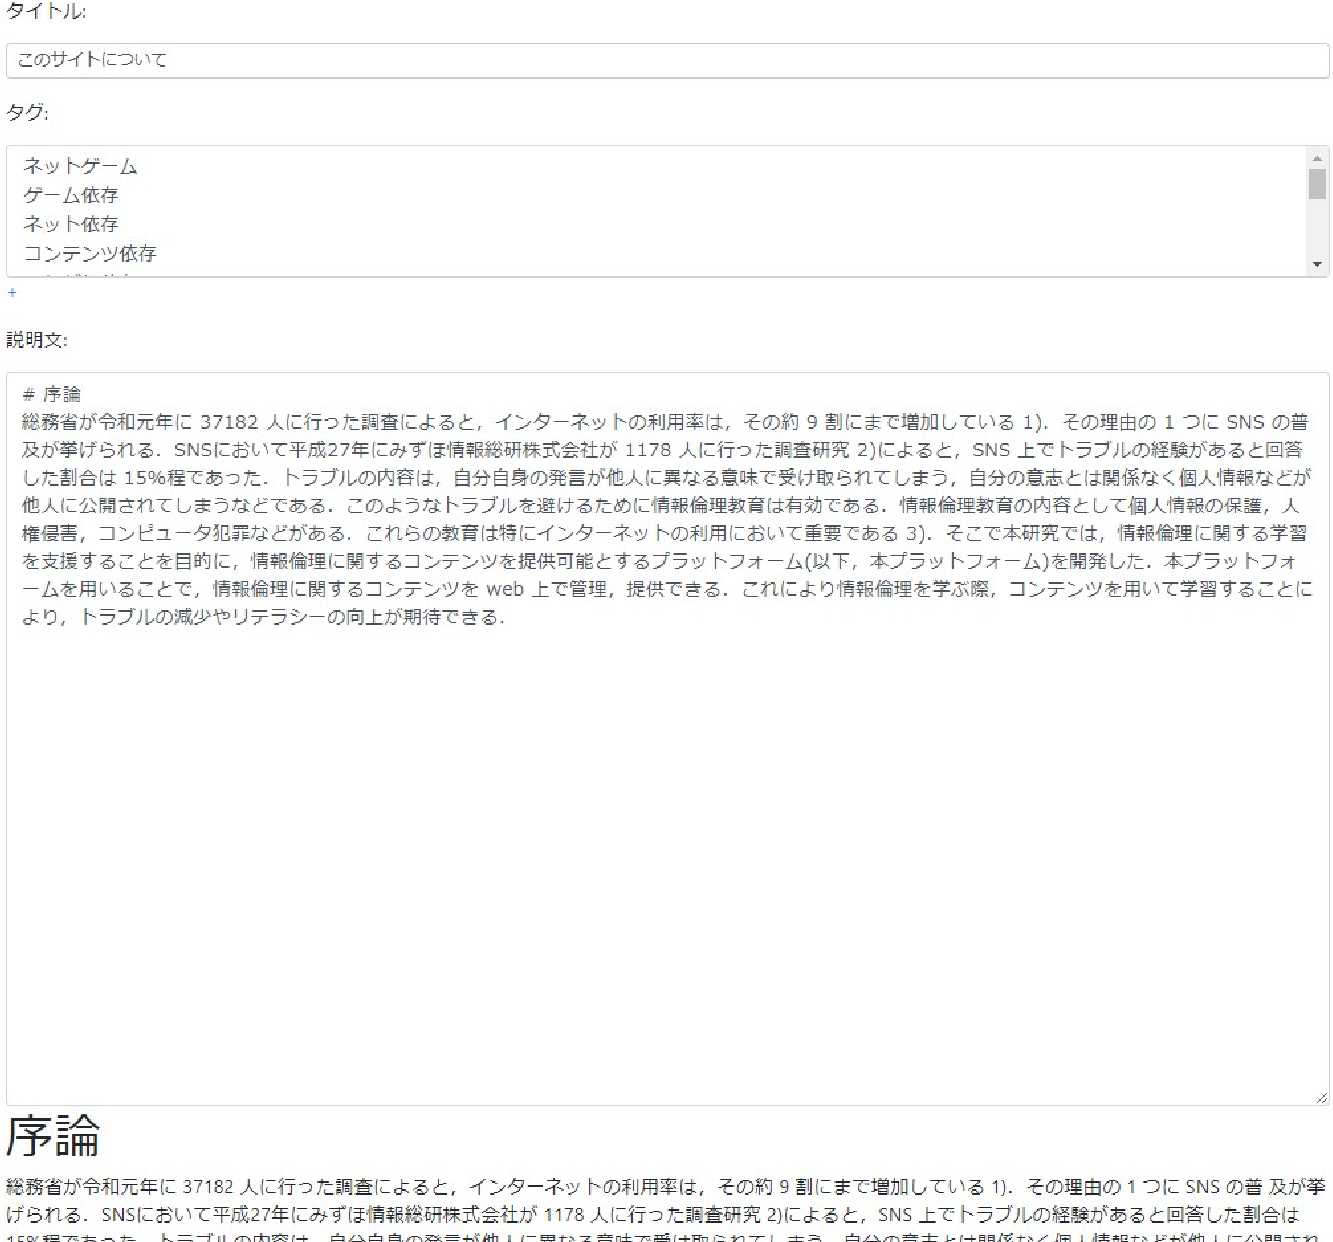
\includegraphics[width=16cm,height=15cm,keepaspectratio]{content_teikyou-crop.pdf}\\
        %includegraphicsの詳しい使い方ははLaTeXの参考書を参照.
    \end{center}
    \caption{コンテンツ提供機能のGUI}
    \label{content_teikyou}
\end{figure}

\newpage
コンテンツのタグは図\ref{content_teikyou}に示すプラスボタンを押下することにより,別画面で新たなタグを登録できる.
タグを登録するときのGUIを図\ref{tag}に示す.
\begin{figure}[htbp]
    \begin{center}
        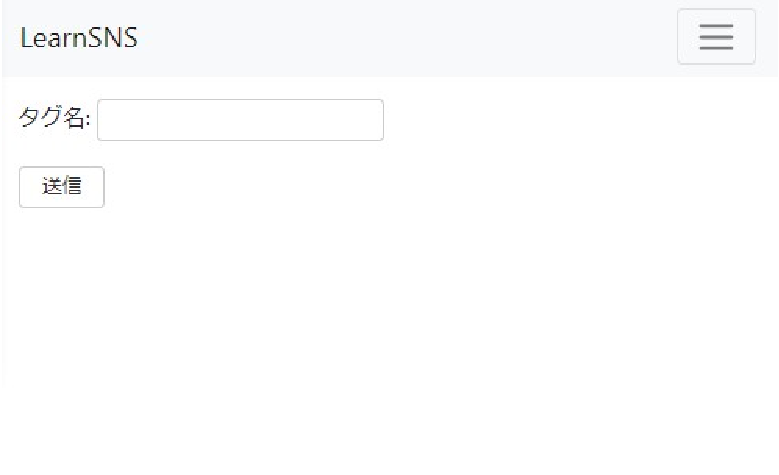
\includegraphics[width=13cm,height=12cm,keepaspectratio]{tag-crop.pdf}\\
        %includegraphicsの詳しい使い方ははLaTeXの参考書を参照.
    \end{center}
    \caption{タグ登録のGUI}
    \label{tag}
\end{figure}

\newpage
また,教材提供者はコンテンツを管理するためのグループに参加する.
そのグループはすべてのコンテンツに対して公開または非公開を選択することでコンテンツを管理する.
グループに参加している教材提供者全員が認可したコンテンツのみが学習者に公開される.
これにより,コンテンツの正当性を担保できる.
教材提供者をグループに参加させるには,図\ref{group_register}のようにして教材提供者のアカウントを選択し教材提供者のグループに登録する.

\begin{figure}[htbp]
    \begin{center}
        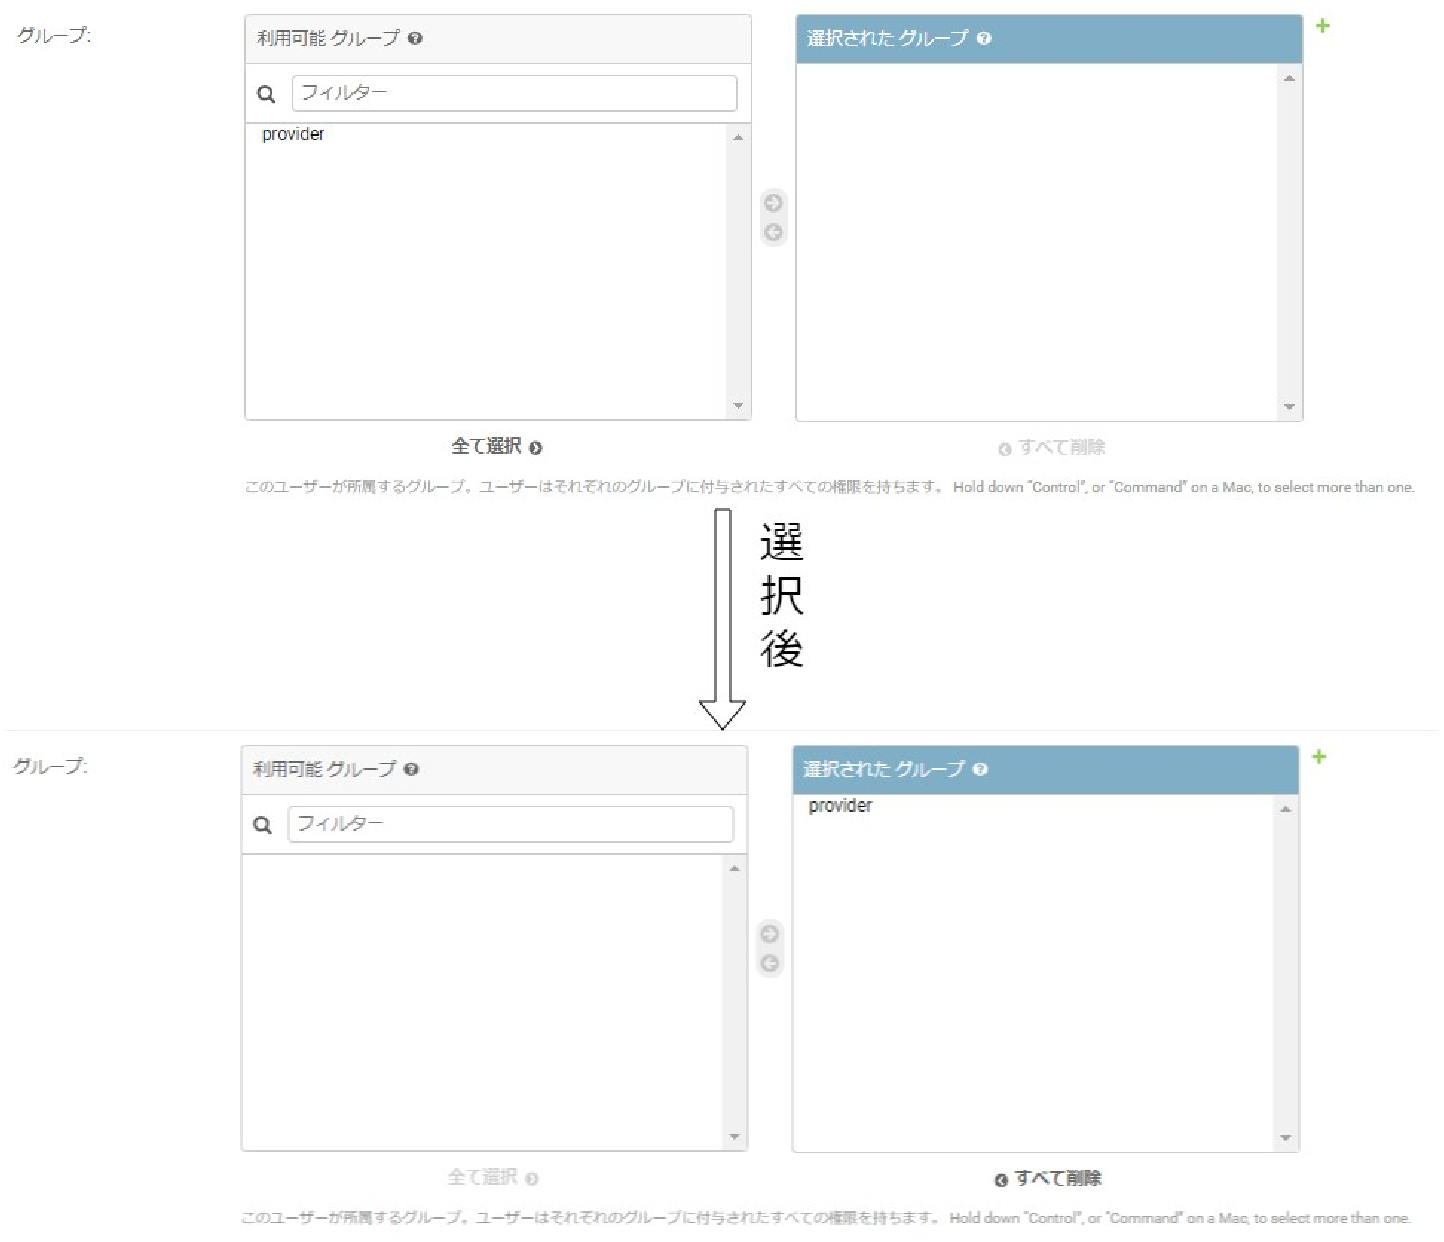
\includegraphics[width=16cm,height=15cm,keepaspectratio]{group_register-crop.pdf}\\
        %includegraphicsの詳しい使い方ははLaTeXの参考書を参照.
    \end{center}
    \caption{グループ登録のGUI}
    \label{group_register}
\end{figure}

\newpage
続いて本機能ではコンテンツ作成後にコンテンツの4択問題を作成することができる.問題の作成には,問題のタイトル,問題文,選択肢1~4および正解の選択肢をフォームに従って入力する.
問題作成時のGUIを図\ref{create_question}に示す.

\begin{figure}[htbp]
    \begin{center}
        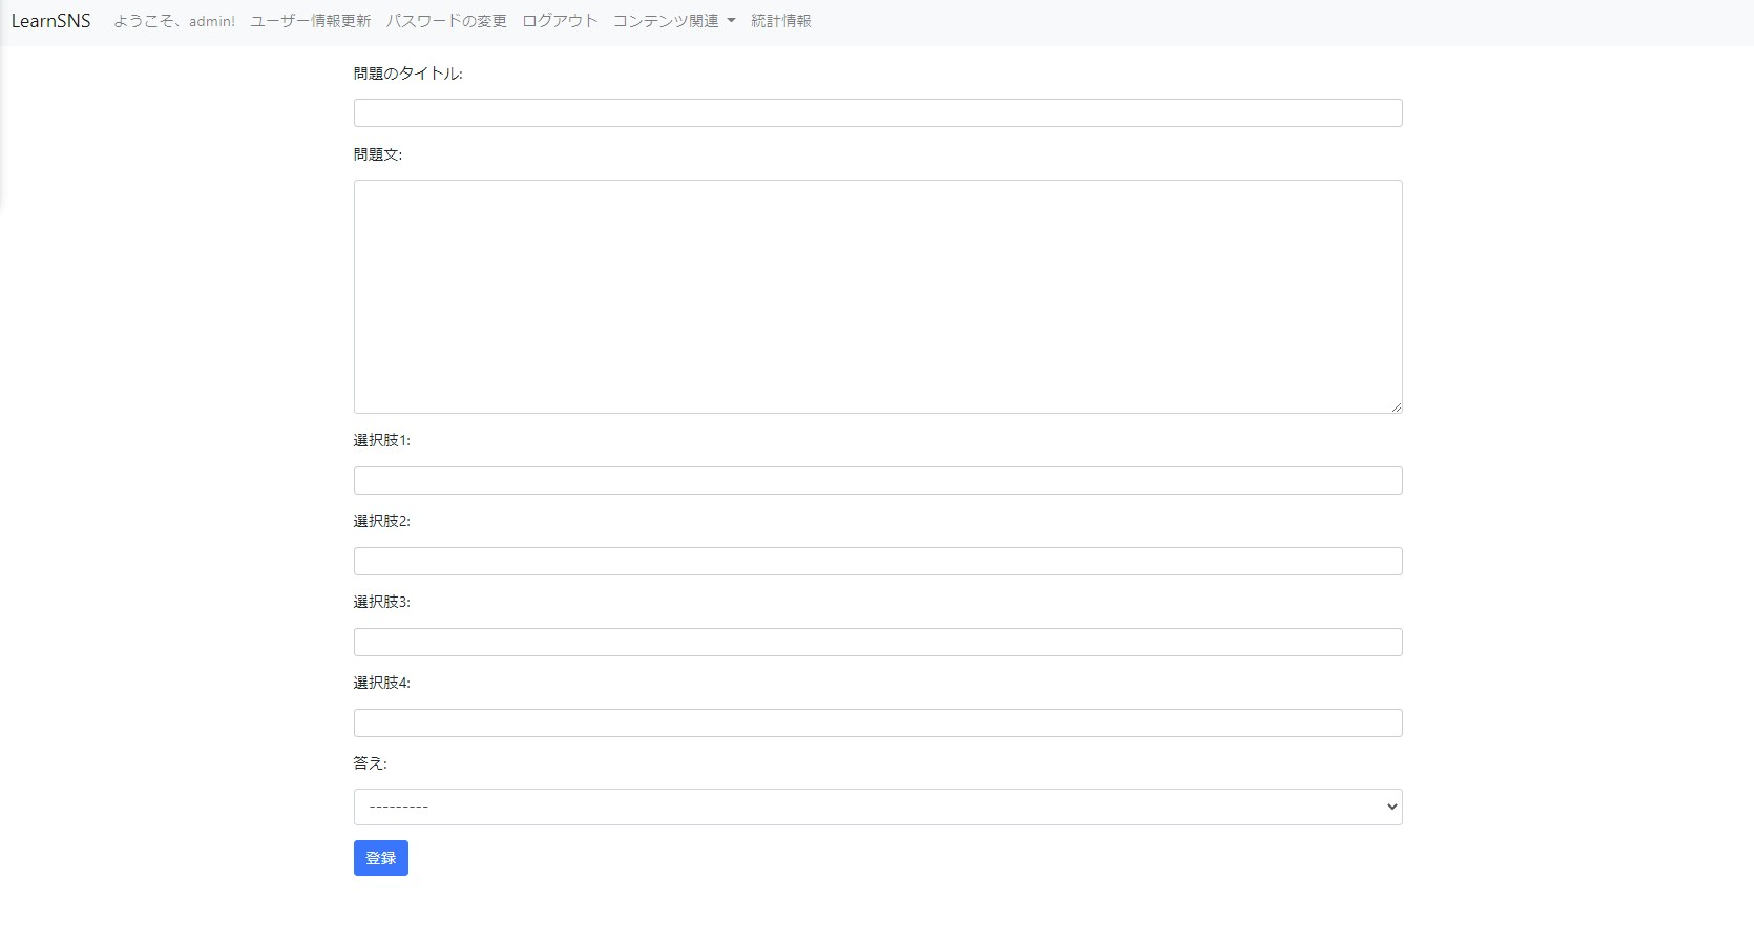
\includegraphics[width=18cm,height=17cm,keepaspectratio]{create_question-crop.pdf}\\
        %includegraphicsの詳しい使い方ははLaTeXの参考書を参照.
    \end{center}
    \caption{問題作成のGUI}
    \label{create_question}
\end{figure}

最後に,Djangoの機能を用いることにより本機能で投稿したコンテンツをJsonファイルに変換することができる.
Jsonファイルに変換するには,以下のような手順を経てコマンドを発行すればよい.
これにより,教材提供者はコンテンツを互いにJsonファイルを介して共有することが可能となる.

\begin{enumerate}
    \item 「docker exec -it コンテナ名 /bin/ash」などとして,本プラットフォームを動作させているコンテナにログインする.
    \item cdコマンドを用いてDjangoによって自動的に生成されたmanage.pyファイルと同階層に移動する.
    \item 「python manage.py dumpdata Jsonファイルに変換したいデータのDBのテーブル名 \textgreater 保存するJsonファイル名.json」を実行後,Jsonファイルが生成される.
\end{enumerate}